\section{Minimum Column Removal}

The problem of removing some columns so that the remaining columns have a perfect phylogeny has been widely studied in the literature (cit. Tomescu) and is is usually modeled as finding an independent set of the conflict graph.

In the case of persistent phylogeny this approach cannot be used since there is no induced submatrix.

Now, a complex red-black graph is characterized by the fact that it induces a
conflict-graph with more than one non trivial component as proved in 
Lemma~\ref{lem:twoComp}.

More precisely,  we show that every successful
reduction of  $G_{RB}$ starts with the realization of a set of
characters with special properties and tree $T$ has also a special structure.
In fact, each tree $T$ consists of  $k \geq 2$ subtrees $T_1, \cdots, T_k$
such that there exists a unique path, called \emph{split path}, from root $r$
of $T$ to a node $x$ (called the \emph{end} of the split path)
that is  the root of all  trees $T_1, \cdots, T_k$.
The set of characters labeling a split path is called a {\em split set} for
$G_{RB}$.
Notice that the split set contains only positive characters (otherwise we would
have a null
character in $\grb$) that are negated in some edge of $T$ (otherwise we would
have a universal character).
\begin{comment}
Then the realization of $C'$ divides the red-black graph into $k$ distinct
components each representing a subtree $T_i$ of tree $T$.  Moreover,  after the
realization of set
$C'$  in the red-black graph,  the   conflict-graph induced by the new
red-black graph  has no
conflicting-pair including characters of $C'$ ($C'$ is a {\em conflict-free
  split set}).
\end{comment}

Our main characterization of complex red-black graphs follows.

\begin{lemma}
  \label{lem:twoComp}
Let $M_e$ be an extended matrix whose red-black graph  $G_{RB}$
is connected, complex and solved by a standard tree $T$.
Then $G_{c}$ has  at least two non trivial
connected components.
\begin{comment}
 $G_{c_1} \cdots G_{c_k}$ with $k \geq 2$.
and the tree $T$
consists of a unique path from the root to a node $x$ such that the label
sequence for node $x$ split the red-black graph into at least two disjoint
red-black graphs.
\end{comment}
\end{lemma}


\begin{proof} % (of Lemma~\ref{lem:twoComp})
Since \grb is connected, there is a split path ending in a node $x$. and let
$X$ be the corresponding split set.
We already know that each character in
$X$ must be negated in $T$.

Let $T_{1}$ be a generic subtree of $T$ and let $S_{1}$ be its set of species.
First we notice that if a character $c^{+}$ appears in $T_{1}$, then
$\me[c^{+},s]=\me[c^{-},s]=0$ for each species $s$ in any other subtree of $T$.
Consider now the case where the character $c^{+}$ appears in $X$ and $c^{-}$
appears in $T_{1}$; in this case $\me[c^{+},s]=1$, $\me[c^{-},s]=0$ for each
species $s$ in any other subtree of $T$.
By the generality of $T_{1}$, all characters that change state in one of the
other subtrees cannot change state in $T_{1}$.
This fact make impossible to have two conflicting characters labeling edges of
two different subtrees, hence no connected component of $G_{c}$ spans characters
appearing in two different subtrees.

Now we are going to prove that there are at least two nontrivial connected
components of $G_{c}$.
Assume to the contrary that that $T$ is a counterexample with the minimum number
of negated characters.
Notice now that each subtree has at least an edge labeled by a negated
character, for otherwise there would be a species that can be realized,
contradicting the hypothesis that \grb is complex
Since there are at least two subtrees $T_{1}$ and $T_{2}$, w.l.o.g. we can
assume that $c_{1}^{-}$ appears in $T_{1}$ and $c_{2}^{-}$ appears in $T_{2}$.
By minimality of the number of negated characters and the first part of the
proof, both $c_{1}$ and $c_{2}$ are involved in two different conflicts that are
edges of two different connected components of $G_{c}$.
Since both components have an edge, they are nontrivial.
\end{proof}




\subsection{A characterization of matrices without a pp tree solution}


Now, given
an incomplete extended matrix $M_e$ associated to a red-black graph,  the
matrix $Grid$  has an entry $ [e, ij]$ for each edge $e= (x,y)$ of the
conflict-graph  and configuration $ij$  for the characters $x$ and $y$ of edge
$e$. Then entry $Grid[e, ij]$ reports the chains of species (rows of matrix
$M_e$)  in poset $(P,<_s)$ that induce the configuration $ij$ for edge $e$.
Then a \initial positive path-sequence is identified by merging entries (i.e
chains) of the grid-matrix $Grid[e, ij]$.  In fact, observe that  the  entry of
$Grid[e, ij]$ consists of  species that once they are solved in the red-black
graph, i.e. they become isolated nodes in the red-black graph. Consequently,
the rows corresponding to  the configuration $ij$
they induce in the original matrix $M$, are  removed from $M$. It follows that
the edge $e$ is not present in the  conflict-graph induced in $M$ by the rows
and columns
that are in the connected red-black graph (see Definition
\ref{def:conflict-induced-by-red-black}).


Let  $Grid$ be the grid of a conflict graph $G_{c}$ and  let $e=(x,y)$ be an
edge of $G_{c}$.
Let $Good(e)$  be  the union of all species that are in the entries
$Grid[e,ij]$ for $ij \in \{10,01,00\} $.
\begin{lemma}\label{lem-inters-vuota}
  Assume that the conflict  graph  $G_c$   for the binary matrix $M$ is formed
by only one non trivial connected component and the red-black graph $G_{RB}$
for $M$ is connected. Assume that
  $\bigcap_{e \in E(G_c)} Good(e) = \emptyset$.
  Then $M$ does not admit a persistent perfect phylogeny.
\end{lemma}
\begin{proof}
  First let us assume that all universal characters have been realized in the
red-black graph $G_{RB}$, thus the matrix $M$ has no universal character.

  By applying Lemma~\ref{lem:twoComp}, it must be that the conflict graph
consists
  of at least two non trivial connected components, thus obtaining a
contradiction.


\end{proof}



By Lemma~\ref{lem-inters-vuota} we can show that exists a infinite set of
matrix that do not admit a p-pp tree. These matrices have associated a
connected conflict graph that is an unchordal cycle and $\bigcap_{e \in E(G_c)}
Good(e) = \emptyset$.


\begin{theorem}
  \label{teo_esistenza_PM}
  For each $n \ge 4$ exists a $n \times n$ forbidden matrix which does not
admit persistent perfect phylogeny and such
  that it does not contain a smaller forbidden matrix.
  % Exists an infinite set $P_M$ of $n \times n$ forbidden distinct matrix, with $n \ge 4$, wherdove per matrici distinte si intende che $\forall M, M' \in P_M$, $M$ non è una sotto-matrice indotta da $M'$ e viceversa, che non ammettono filogenesi perfetta persistente.
\end{theorem}
\begin{proof}
  For each $n\ge 4$, $\exists$ a $n \times n$ binary matrix $M$, such that
$\forall$ $1 \le i < n$ the species at the row $i$ has the pair of characters
$(c_i, c_{i+1})$ and the species at the row $n$ has the pair $(c_1, c_n)$.

  By construction $M$ has associated an unchordal cycle conflict graph $G_c$
and such that $\bigcap_{e \in E(G_c)} Good(e) = \emptyset$. Consequently by the
Lemma~\ref{lem-inters-vuota} the matrix $M$ does not admit persistent perfect
phylogeny.

\end{proof}




\subsection{Examples}

The following matrix $M$ admits a pp tree but has no path-sequence.

\begin{figure}[htbp]
$$
     {\mathcal M} =
     \begin{array}{c|cccccccccccccccc}
     s/c & c_1 & c_2 & c_3 & c_4 & c_5 & c_6 & c_7 & c_8 & c_9 & c_{10} &
c_{11} & c_{12} & c_{13} & c_{14} & c_{15} & c_{16}\\
     \hline
     1 & 1 & 1 & 1 & 0 & 0 & 0 & 1 & 0 & 1 & 0 & 0 & 0 & 0 & 0 & 0 & 0 \\
	 2 & 1 & 1 & 1 & 0 & 0 & 0 & 1 & 1 & 0 & 1 & 0 & 0 & 0 & 0 & 0 & 0 \\
	 3 & 1 & 1 & 0 & 1 & 0 & 0 & 1 & 1 & 0 & 0 & 1 & 0 & 0 & 0 & 0 & 0 \\
	 4 & 1 & 1 & 0 & 1 & 0 & 0 & 0 & 1 & 0 & 0 & 0 & 1 & 0 & 0 & 0 & 0 \\
	 5 & 1 & 0 & 1 & 1 & 1 & 0 & 0 & 0 & 0 & 0 & 0 & 0 & 1 & 0 & 0 & 0 \\
	 6 & 1 & 0 & 1 & 1 & 1 & 1 & 0 & 0 & 0 & 0 & 0 & 0 & 0 & 1 & 0 & 0 \\
	 7 & 0 & 1 & 1 & 1 & 1 & 1 & 0 & 0 & 0 & 0 & 0 & 0 & 0 & 0 & 1 & 0 \\
	 8 & 0 & 1 & 1 & 1 & 0 & 1 & 0 & 0 & 0 & 0 & 0 & 0 & 0 & 0 & 0 & 1 \\
      \end{array}
$$
\caption{A binary matrix  $M$ of size  $8 \times 16$ admitting a persistent
tree}
\label{fig:matAmmetteP-pp}
\end{figure}

\begin{figure}[htbp]
\centering
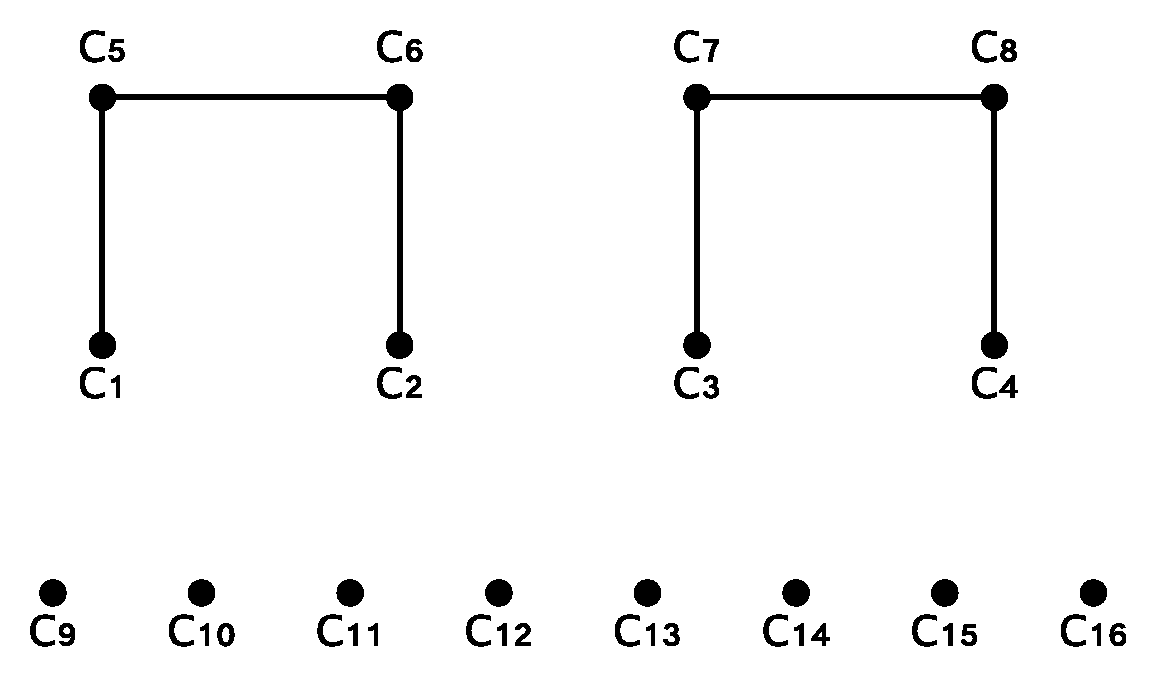
\includegraphics[height=10cm, width=8cm,keepaspectratio]{GrafoConflitti1}
\caption{Conflict graph associated to the matrix  $M$ given in Fig.
\ref{fig:matAmmetteP-pp} }
\label{fig:GcM}
\end{figure}


 Figure~\ref{fig:GcM} illustrates the conflict graph of matrix $M$. It consists
of two non trivial connected components and singletons.
\\
It is immediate to verify that the red-black graph for matrix $M$ does not have
a species $s$ that can be realized, as  $\bigcap_{e \in E(G_c)}Good(e) =
\emptyset$.
Moreover observe that all species are not comparable under the $<_s$-relation.
The red-black graph  for $M$   admits a successful reduction   $r $ given by
the sequence $\langle c_1, c_2, c_3, c_4, c_5, c_6, c_7, c_8, c_{13}, c_{14},
c_{15}, c_{16}, c_9, c_{10}, c_{11}, c_{12} \rangle$.
The persistent phylogeny for matrix $M$ is given in Figure ~\ref{fig:albero1}.



A similar problem can be defined when we also have a topology T in input.

Special case: the input matrix has a perfect phylogeny on T and we want a persistent phylogeny. In that case a matching on the conflict graph suffices.

Also maximization version, where we want to maximize the number of columns that are kept.

Notice that allowing only the removal of some rows does not really make sense if only leaves of T can be labeled by some species.
